This chapter presents the language definition and compiler architecture of Metacasanova. 


\section{Repetitive steps in compiler development}
\label{sec:ch_metacasanova_intro}
In Chapter \ref{ch:background} we gave on overview of the necessary steps involved in developing a compiler. We showed that the lexing/parsing phase is simple enough to be automated using a lexer/parser generator. Such software takes as input the grammar and the definitions of regular expressions to define the tokens of the language and produces output code containing that is able to parse a program written in a programming language defined by that grammar. However, the steps involved in the following phases, namely the \textit{type checking} and \textit{operational semantics} implementation follow a recurring pattern, but in general the behaviour of the type system and the code generation reflecting the behaviour of the operational semantics must be hard-coded in the host language in which the compiler is being implemented. Below we present two examples to show how these behaviours can be implemented in two different general purpose programming languages and show that both follow the same pattern.

\subsection{Hard-coded implementation of type rules}
\label{sec:ch_metacasanova_hc_type_rules}
As shown in Section \ref{sec:ch_background_type_checking}, type rules are expressed in the form of logical rules. Let us consider the type rules for the \texttt{if-then-else} and \texttt{while-do} statements presented in Section \ref{sec:ch_background_type_checking} in the version that assigns the type \textit{unit} to the code blocks for convenience. In a programming language that supports discriminated unions as a language abstraction (like Haskell or F\#), the syntactical element in the abstract syntax tree of the language can be expressed as

\begin{lstlisting}
type Statement =
| If of Expr * List<Statement> * List<Statement>
| While of Expr * List<Statement>
... //other statements
\end{lstlisting}

The type checking of the \texttt{if} statement requires that to check that the condition has type \texttt{bool} and that both code blocks have type \texttt{unit} (or \texttt{void}). The type checking of the \texttt{while-do} is analogous, except only one code block is used. We can then define a function \texttt{eval} that, given the environment (here we call it \textit{symbol table}) and a statement as input, returns the type given by the rule or an error if all type rules for that statement fail to correctly evaluate. For the 
\texttt{if-then-else} the implementation is the following:

\begin{lstlisting}
let rec evalStmt (symbolTable : SymbolTable) (stmt : Statement) : Type =
match stmt with
... //other statements
| If (condition,_then,_else) ->
    let conditionType = evalExpr symbolTable condition
    let thenType = evalStmt symbolTable _then
    let elseType = evalStmt symbolTable _else
    if conditionType <> Boolean then
      failwith "Invalid condition type"
    elif thenType <> Unit then
      failwith "The type of then must be unit"
    elif elseType <> Unit then
      failwith "The type of else must be unit"
    else
      Unit
... //other statements
\end{lstlisting}

\noindent
The function first executes pattern matching on the statement to identify the correct inference rule to use during the typing. It then proceeds to evaluate the premises (type of the condition and of the statement blocks) and to check their result. If all premises evaluate successfully the type contained in the conclusion is returned. Note that the function \texttt{evalExpr} is a function able to evaluate the type rule for expressions and return their type. 
The implementation of the \texttt{while-do} follows the same logic:

\begin{lstlisting}
let rec evalStmt (symbolTable : SymbolTable) (stmt : Statement) : Type =
match stmt with
... //other statements
| While (condition,_do) ->
  let conditionType = evalExpr symbolTable condition
  let doType = evalStmt symbolTable stmt
  if conditionType <> Boolean then
    failwith "Invalid condition type"
  elif doType <> Unit then
    failwith "The type of the do block must be unit"
  else
    Unit
... //other statements
\end{lstlisting}

In languages that do not provide abstractions such as discriminated unions, the type for statements must exploit polymorphism to implement the same behaviour. A statement will be represented as an interface exhibiting the behaviour of a visitor pattern:

\begin{lstlisting}
public interface Statement
{
  Type Visit(StatementVisitor visitor);
}

public interface StatementVisitor
{
  ... //other statements
  Type OnIf(Expression condition, List<Statement> _then, List<Statement> _else);
  Type OnWhile(Expression condition, List<Statement> _do);
  ... //other statements
}
\end{lstlisting}

The behaviour of the inference rule for the \texttt{if-then-else} statement is modelled by a class implementing the \texttt{StatementVisitor} interface. This class contains a method \texttt{OnIf} that implements the behaviour of the type rule itself. 

\begin{lstlisting}
public class StatementEvaluator : StatementVisitor
{
  ... //evaluation of other statements
  public Type OnIf(Expression condition, List<Statement> _then, List<Statement> _else)
  {
    Type conditionType = condition.visit(new ExpressionEvaluator());
    Type thenType = _then.Visit(new StatementEvaluator());
    Type elseType = _else.Visit(new StatementEvaluator());
    if (!conditionType.Equals(new Boolean()))
    {
      throw new TypeException("Invalid condition type");
    }
    else if (!thenType.Equals(new Unit()))
    {
      throw new TypeException("The type of then must be unit");
    }
    else if (!elseType.Equals(new Unit()))
    {
      throw new TypeException("The type of else must be unit");
    }
    else
    {
      return new Unit();
    }
  }
  
  ... //evaluation of other statements
}

public class If : Statement
{
  Expression Condition;
  List<Statement>  Then;
  List<Statement> Else;
  
  public Type Visit(StatementVisitor visitor)
  {
    return visitor.OnIf(this.Condition, this.Then, this.Else)
  }
}
\end{lstlisting}

Analogously for the \texttt{while-do} we have

\begin{lstlisting}
public class StatementEvaluator : StatementVisitor
{
  ... //evaluation of other statements
  public Type OnWhile(Expression condition, List<Statement> _do)
  {
    Type conditionType = condition.Visit(new ExpressionEvaluator());
    Type doType = _do.Visit(new StatementEvaluator());
    if (!conditionType.Equals(new Boolean()))
    {
      throw new TypeException("Invalid condition type");
    }
    else if (!doType.Equals(new Unit()))
    {
      throw new TypeException("The type of do must be unit");
    }
    else
    {
      return new Unit();
    }
  }
  ... //evaluation of other statements
}

public class While : Statement
{
  Expression Condition;
  List<Statement> Do;
  
  public Type Visit(StatementVisitor visitor)
  {
    return visitor.OnWhile(this.Condition, this.Do);
  }
}
\end{lstlisting}

\subsubsection{Generalization}
\label{sec:ch_metacasanova_inference_rule_generalization}

In general, for a node of the abstract syntax tree (AST) $\alpha$ (like \texttt{Statements}) containing syntactical structures $\sigma_{i}$ constructed with a certain amount of arguments of type $\epsilon_{\sigma_{i_1}}, ..., \epsilon_{\sigma_{i_m}}$ (such as the condition or the statement block in a control structure), the general representation of a hard-coded type rule in a language with discriminated unions is obtained by creating a union type $\alpha$ having a case $\sigma_{i}$ with arguments $\epsilon_{\sigma_{i_j}}$ for each syntactical element.

\begin{lstlisting}[mathescape = true]
type $\alpha$ =
|$\sigma_1$ of $\tau_{\sigma_{1_1}} * ... * \tau_{\sigma_{1_m}}$
...
|$\sigma_n$ of $\tau_{\sigma_{n_1}} * ... * \tau_{\sigma_{n_m}}$
\end{lstlisting}

Evaluating the inference rule through an evaluation function requires first to find out which must be applied by matching the pattern of the syntactical structure from the node of the AST. Later, we need to evaluate each of the premises with the appropriate evaluation function: if the result of each evaluation is what the rule expects (for instance, that the condition has type boolean in the \texttt{if-then-else}) then we return the result of the evaluation rule contained in the right part of the conclusion.

Let us consider a conclusion $\sigma_{j}(\epsilon_{\sigma_{j_1}} \; ... \;\epsilon_{\sigma_{j_m}})$ (where each $\epsilon$ is one of the arguments used to construct the case of the discriminate union) with a result of the evaluation $\rho_{\sigma_j}$ a set of premises $\pi_{1},...,\pi_{k}$ that are evaluated through an evaluation function $\varphi_{\pi_i}, \; i = 1,...,k$ returning a result $\rho_{\pi_i}$. Let us assume that $\rho'_{\pi_i}$ is the expected result for the premise evaluated through $\varphi_{\pi_i}$. As usual, $\Gamma$ defines the environment (symbol table). The type rule that we are trying to execute will thus have the following structure:

\begin{mathpar}
	\mprset{flushleft}
	\inferrule*
	{\Gamma \vdash \varphi_{\pi_1} \pi_1 : \rho'_{\pi_1} \\\\
	\vdots \\\\
	\Gamma \vdash \varphi_{\pi_i} \pi_i : \rho'_{\pi_i} \\\\
	\vdots\\\\
	\Gamma \vdash \varphi_{\pi_k} \pi_k : \rho'_{\pi_k}}
 {	\Gamma \vdash \sigma_{j}(\epsilon_{\sigma_{j_1}},...,\epsilon_{\sigma_{j_m}}) : \rho_{\sigma_j}} \\
\end{mathpar}

Given the considerations above, the code necessary for the evaluation will be the following:

\begin{lstlisting}[mathescape = true]
let rec $\varphi_{\sigma_j}$ $\Gamma$ $\sigma$ =
  match $\sigma$ with
  ... //other pattern matching expressions for other rules
  | $\sigma_{j}(\epsilon_{\sigma_{j_1}},...,\epsilon_{\sigma_{j_m}})$ ->
    let $\rho_{\pi_1}$ = $\varphi_{\pi_1}$ $\Gamma$ $\pi_1$
    .
    .
    .
    let $\rho_{\pi_i}$ = $\varphi_{\pi_i}$ $\Gamma$ $\pi_i$
    .
    .
    .
    let $\rho_{\pi_k}$ = $\varphi_{\pi_k}$ $\Gamma$ $\pi_k$
    if $\rho_1$ <> $\rho'_1$ then
      failwith "Type error"
    .
    .
    .
    elif $\rho_i$ <> $\rho'_i$ then
      failwith "Type error"
    .
    .
    .
    elif $\rho_m$ <> $\rho'_m$ then
      failwith "Type error"
    else
      $\rho_{\sigma_j}$    
  ... //other pattern matching expressions for other rules
\end{lstlisting}

Each evaluation function is recursive because a premise might need to run the same evaluation function (see the example of the statements above). The function contains a pattern matching that selects the correct inference rule to be used for that syntactical structure. For example, in the case of the statements, it will try to match all the possible syntactical structures for the statements and select the correct one for the input; for instance, if we are running the rule for the \texttt{if-then-else} then the pattern matching will select the match case for \texttt{if-then-else}. Note that $\gamma$ will surely be matched by one of the match cases because at this point we have a correctly generated AST after the parsing phase.

Each premise runs the appropriate evaluation function and returns a result. This result is compared with the one expected by the inference rule, and if the comparison fails the function reports a type error. If all comparisons succeed, then the result of the conclusion is returned.

In a language that does not provide discriminated unions and pattern matching the generalization is more complex: the abstract syntax tree element must be represented by an interface containing the signature of a method \texttt{Visit} used to perform an operation on a specific (polymorphic) syntactical structure. We also require the interface for the visitor pattern with the signature of the functions to run for each polymorphic instance of \texttt{Statement}. In this version we assume that the type of the result of the evaluation function for $\sigma_j$ returns a type $\tau_{\rho_{\sigma_{j}}}$ (which in the previous version could be omitted thanks to the type inference typical of functional programming languages):

\begin{lstlisting}[mathescape = true]
public interface $\alpha$
{
  public $\tau_{\sigma_j}$ Visit(Visitor visitor)
}

public interface Visitor<T>
{
  T $\varphi_{\sigma_j}(\tau_\Gamma \; \Gamma, \tau_{\sigma_{j_1}} \epsilon_{\sigma_{j_1}},...,\tau_{\sigma_{j_m}}\epsilon_{\sigma_{j_m}})$;
  ... //other statements
}
\end{lstlisting}

\noindent
Then we have to implement the visitor for the type rule for statements and a class for a specific statement:

\begin{lstlisting}[mathescape = true]
public class Evaluator : Visitor<$\tau_{\rho_{\sigma_{j}}}$>
{
  ... //evaluation of other statements
  public $\tau_{\rho_{\sigma_{j}}}$ $\varphi_{\sigma_j}(\tau_\Gamma \; \Gamma, \tau_{\sigma_{j_1}}\epsilon_{\sigma_{j_1}},...,\tau_{\sigma_{j_m}}\epsilon_{\sigma_{j_m}})$
  {
    $\tau_{\rho_{\phi_1}} \rho_{\pi_1}$ = $\varphi_{\pi_1}(\Gamma,\pi_1)$;
    .
    .
    .
    $\tau_{\rho_{\phi_i}} \rho_{\pi_i}$ = $\varphi_{\pi_i} (\Gamma,\pi_i)$;
    .
    .
    .
    $\tau_{\rho_{\phi_k}} \rho_{\pi_k}$ = $\varphi_{\pi_k}( \Gamma,\pi_k)$
    if (!$\rho_{\pi_1}$.Equals($\rho'_{\pi_1})$)
      throw new TypeError("Type error");
    .
    .
    .
    else if (!$\rho_{\pi_i}$.Equals($\rho'_{\pi_i})$)
      throw new TypeError("Type Error");
    .
    .
    .
    else if (!$\rho_{\pi_k}$.Equals($\rho'_{\pi_k})$)
      throw new TypeError("Type Error");
    else
      return new $\rho_{\sigma_j}$();
  }
  ... //evaluation of other statements
}

public $\sigma_j$ : $\alpha$
{
  $\tau_{\sigma_{j_1}} \epsilon_{\sigma_{j_1}}$;
  ...
  $\tau_{\sigma_{j_m}} \epsilon_{\sigma_{j_m}}$;
  
  public $\tau_{\rho_{\sigma_{j}}}$ Visit(Visitor<$\tau_{\rho_{\sigma_{j}}}$> visitor)
  {
    return visitor.$\varphi_{\sigma_j}$($ \epsilon_{\sigma_{j_1}},...,\epsilon_{\sigma_{j_m}}$);
  }
}
\end{lstlisting}

A general pseudo-code representation of the rule evaluation is shown in Algorithm \ref{alg:ch_metacasanova_rule_evaluation}.

\begin{algorithm}
	\caption{Pseudocode of rule evaluation}
	\label{alg:ch_metacasanova_rule_evaluation}
	\begin{algorithmic}
		\Function{Evaluate rule}{$R \text{ inference rule }$, $I \text{ input of the rule }$}
		\If {$\text{\textbf{not }} R.Conclusion \text{ matches } I$}
			\State \Return $\text{\textbf{error}}$
		\EndIf
		\ForAll {$p \text{ in } R.Premises$}
		  \State $p'\gets \text{textbf{ evaluate }} p$
		  \If {$\text{\textbf{not }}p.Result \text{\textbf{ matches }} p$}
		    \State \Return $\text{\textbf{error}}$
		  \EndIf
		\EndFor
		\State \Return $R.Result$
		\EndFunction
	\end{algorithmic}
\end{algorithm}

A graphical representation of the rule evaluation can be found in Figure \ref{fig:ch_metacasanova_rule_evaluation}.

\begin{figure}
	\centering
	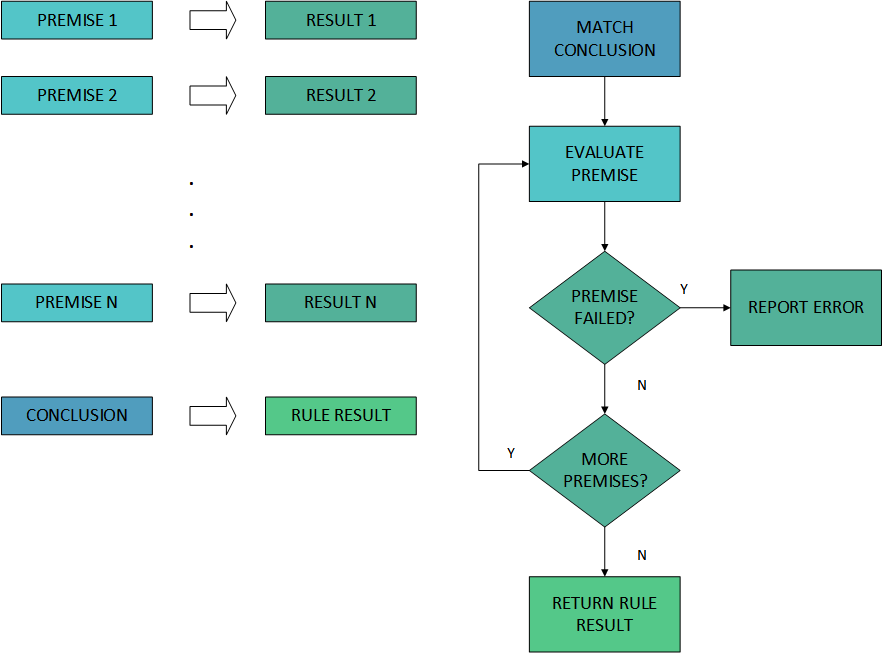
\includegraphics[width = \textwidth]{Figures/chapter_metacasanova/rule_evaluation}
	\caption{Diagram of rule evaluation: on the left side the structure of an inference rule, on the right side its evaluation expressed as a flow chart. The components of the rule are coloured to match the parts in which they are used in the flow chart.}
	\label{fig:ch_metacasanova_rule_evaluation}
\end{figure}

\subsection{Hard-coded implementation of Semantics}
\label{sec:ch_metacasanova_hc_semantics}
As shown in Section \ref{sec:ch_background_semantics}, there are multiple ways to express the semantics of a programming language. In this work we choose to make use of the operational semantics representation to have a uniform way of expressing both the type system and the semantics of a language. Let us consider again the semantics rule for \texttt{if-then-else} and \texttt{while-do} presented in Section \ref{sec:ch_background_semantics}. The operational semantics can be implemented generating the code in the object language that emulates the behaviour of the semantics rule, in the same fashion of a type rule. This process might first pass through an intermediate language, closer to the target language. In the case of an interpreter, the behaviour of the semantics must be implemented using the abstractions available in the host language. As an example, we show a possible implementation of the semantics of the two statements mentioned above in an interpreter both in a functional programming language and in an object-oriented language, as for the type rule.

For convenience, let us make a separate rule for the semantics of a sequence of statements from the specific semantics of the control structure. Also, we introduce the statement \texttt{skip} that performs no operation

\begin{mathpar}
	\mprset{flushleft}
	\inferrule*
	{ }
	{\langle \text{skip} ; ks \rangle \Rightarrow \langle ks \rangle}
\end{mathpar}
\begin{mathpar}
	\mprset{flushleft}
	\inferrule*
	{\langle k \rangle \Rightarrow k'}
	{\langle k ; ks \rangle \Rightarrow \langle k' ; ks \rangle}
\end{mathpar}
\begin{mathpar}
	\mprset{flushleft}
	\inferrule*
	{\langle c \rangle \Rightarrow \text{\texttt{true}}}
	{\langle \text{if \textit{c} then \textit{T} else \textit{E}} \rangle \Rightarrow \text{\textit{T}}}
\end{mathpar}
\begin{mathpar}	
	\mprset{flushleft}
	\inferrule*
	{\langle c \rangle \Rightarrow \text{\texttt{false}}}
	{\langle \text{if \textit{c} then \textit{T} else \textit{E}} \rangle \Rightarrow \text{\textit{E}}}
\end{mathpar}
\begin{mathpar}	
	\mprset{flushleft}
	\inferrule*
	{\langle c \rangle \Rightarrow \text{\texttt{true}}}
	{\langle \text{while \textit{c} do \textit{L}} \rangle \Rightarrow \text{\textit{L} ; while \textit{c} do \textit{L}}}
\end{mathpar}
\begin{mathpar}	
	\mprset{flushleft}
	\inferrule*
	{\langle c \rangle \Rightarrow \text{\texttt{true}}}
	{\langle \text{while \textit{c} do \textit{L}} \rangle \Rightarrow \text{skip} }
\end{mathpar}

As for the type rules, we assume that the data type representing a statement is implemented by a discriminate union. The evaluation function first performs the pattern matching on the argument to select the correct rule to execute, in the same fashion of the type rule, but instead of analysing the types this time executes the specific behaviour of the statement, as specified by the semantics rule. For inference rules above we use the following code:

\begin{lstlisting}
let rec interpretStmt (symbolTable : SymbolTable) (stmt : Statement) : Statement =
  match stmt with
  ... //other statements semantics
  | Sequence(Skip,ks) -> interpretStmt symbolTable ks
  | Sequence(k,ks) ->
  	 let k' = interpretStmt symbolTable k
  	 interpretStmt symbolTable Sequence(k',ks)
  | If (cond,_then,_else) ->
      let condEvaluation = interpretExpr symbolTable cond
      if condEvaluation = True then
      	_then
      else
        _else
  | While (cond,_do) ->
     let condEvaluation = interpretExpr symbolTable cond
     if condEvaluation = true then
       Sequence(_do,While(cond,_do))
      else
        Skip
  ... //other statements semantics
\end{lstlisting}

As for the type evaluation, we assum that \texttt{interpretExpr} is another function that is able to process expressions and return their value. 

The function matches the kind of statement that we want to execute. In the case of a sequence of statements starting with a skip, we simply return the interpretation of the remaining part of the sequence (we indeed skip to the next statement), otherwise we have to run the first statement and then recursively evaluate the sequence formed by the result of the execution of the statement and the rest of the statements. This is needed, for instance, to correctly evaluate the body of a control structure. The body of each match case is responsible of emulating the intended behaviour described in the semantics of the control structure: the \texttt{if} returns the correct block to execute depending on the boolean value of the condition, instead the \texttt{while} returns either its body followed by the same \texttt{while} loop when the condition is \texttt{true}, otherwise \texttt{skip} to jump past the loop.

In the case of an object-oriented language, it is necessary to add a new implementation of the visitor pattern implementing the behaviour of the semantics for each statement:

\begin{lstlisting}
public class StatementInterpreter : StatementVisitor
{
  ... //other statements semantics
  public Statement OnSequence(SymbolTable symbolTable, Sequence seq)
  {
    Statement k = seq.Head;
    Statement ks = seq.Tail;
    if (k.Equals(Skip))
      return ks.Visit(new StatementInterpreter());
    else
    {
      Statement k1 = k.Visit(new StatementInterpreter());
      Statement seq1 = new Sequence(k1,ks)
      return seq1.Visit(new StatementInterpreter());
    }
  }
  public Statement OnIf(Expression cond, Statement _then, Statement _else)
  {
    Value condValue = cond.Visit(new ExpressionInterpreter());
    if (condValue.Equals(new True()))
      return _then;
    else
      return _else;
  }
  public Statement OnWhile(Expression cond, Statement _do)
  {
    Value condValue = cond.Visit(new ExpressionInterpreter());
    if (condValue.Equals(new True()))
      return new Sequence(_do,new While(cond,_do))
    else
      return new Skip();
  }
  ... //other statement semantics
}
\end{lstlisting}

A further remark is that, for the sake of simplicity, here the interpretation only returns a new statement to execute obtained by processing the current statement, but in a real application it should also return a data structure representing the state of the program.

At this point it is possible to observe that this pattern can be generalized as well in a way analogous to that used for type rules for both implementations, which we omit for brevity.


\subsection{Discussion}
In Section \ref{sec:ch_metacasanova_hc_type_rules} and \ref{sec:ch_metacasanova_hc_semantics} we have shown two implementations, one functional and one object-oriented, of type rules and semantics in a possible hard-coded compiler. We have also shown that the pattern can be generalized in both versions. Indeed, their behaviour must be hard-coded in the language chosen for the compiler implementation, regardless of the fact that the pattern is constantly repeated in every rule. This pattern can be captured in a meta-language that is able to process the type system and operational semantics definition of the language and generates the code in the target language necessary to execute the behaviour of the rules. In the following sections we describe the meta-language for \textit{Metacasanova}, a meta-compiler that is able to read a program written in terms of type system/operational semantics rules defining a programming language, a program written in that language, and output executable code that mimics the behaviour of the semantics. The goal of this language is relieving the programmer from writing boiler-plate code when implementing a compiler for a (Domain-Specific) language.

\section{Metacasanova overview}
\label{sec:ch_metacasanova_metacasanova_overview}
In this section we present the general idea behind Metacasanova. We start by defining the requirements of Metacasanova, then we proceed to give a general overview of the language, and finally we formalize the semantics of the language.

\subsection{Requirements of Metacasanova}
In order to relieve programmers of manually defining the behaviour described in Section \ref{sec:ch_metacasanova_hc_type_rules} and \ref{sec:ch_metacasanova_hc_semantics} in the back-end of the compiler, we propose the following features for Metacasanova:

\begin{itemize}
	\item It must be possible to define custom operators (or functions) and data containers. This is needed to define the syntactic structures of the language we are defining.
	\item It must be typed: each syntactic structure can be associated to a specific type in order to be able to detect meaningless terms (such as adding a string to an integer) and notify the error to the user.
	\item It must be possible to have polymorphic syntactical structures. This is useful to define equivalent ``roles'' in the language for the same syntactical structure; for instance we can say that an integer literal is both a \textit{Value} and an \textit{Arithmetic expression}.
	\item It must natively support the evaluation of semantics rules, as those shown above.
\end{itemize}

We can see that these specifications are compatible with the definition of meta-compiler, as the software takes as input a language definition written in the meta-language, a program for that language, and outputs runnable code that mimics the code that a hard-coded compiler would output.

\subsection{Program structure}
In this section we give an informal idea of how a Metacasanova program is organized. Further ahead this idea is expanded with additional details when we present the implementation details of the parser.  \\\\
A Metacasanova program is mainly organized in three parts:

\begin{enumerate}
	\item \textit{Data and function declarations:} in this part it is possible to specify data structures, that define the syntactic constructs of the language, and functions used to evaluate terms of the language through rules.
	\item \textit{Type equivalence declarations:} in this part it is possible to specify polymorphism through type equivalence by stating that a type $T_1$ is equivalent to another type $T_2$.
	\item \textit{Rule definitions:} in this part the programmer defines the type or semantics rules necessary to describe the type system or behaviour of the abstractions of the programming language.
\end{enumerate}

A data structure or function declaration specifies the types of the arguments to construct the data structure or to pass to the function, their name, and the type of the data structure or the function itself
\begin{lstlisting}
Data Expr -> "+" -> Expr : Expr
\end{lstlisting}

\noindent
Note that Metacasanova allows you to specify any kind of notation for data types in the language syntax, depending on the order of definition of the argument types and the constructor name. In the previous example we used an infix notation. The equivalent prefix and postfix notations would be:

\begin{lstlisting}
Data "+" -> Expr -> Expr : Expr
Data Expr -> Expr -> "+" : Expr
\end{lstlisting}

Optionally, it is possible to specify a precedence priority and the associativity. For example, the following code specifies that the multiplication has a higher precedence over the sum and that both are left-associative.

\begin{lstlisting}
Data Expr -> "+" -> Expr : Expr Priority 0 <|
Data Expr -> "*" -> Expr : Expr Priority 1 <|
\end{lstlisting}

\noindent
A function definition is similar to a data definition but it also has a return type. For instance the following is the evaluation function definition for the arithmetic expression above:

\begin{lstlisting}
Func "eval" -> Expr : Value
\end{lstlisting}

\noindent
A polymorphic data structure is defined through the keyword \texttt{is}, which specifies that a type $T_1$ is equivalent to another type $T_2$. For example the following code specifies that a data structure of type \texttt{Value}, such as a list, can be used also as an expression of type \texttt{Expr}.

\begin{lstlisting}
Data "$l" -> List : Value 
Value is Expr
\end{lstlisting}

Metacasanova also allows to embed C\# code into the language by using double angular brackets. This code can be used to embed .NET types when defining data or functions, or to run C\# code in the rules. For example in the following snippet we define a floating point data which encapsulates a floating point number of .NET to be used for arithmetic computations:

\begin{lstlisting}
Data "$f" -> <<float>> : Value
\end{lstlisting}

\noindent
A rule in Metacasanova may contain a sequence of premises and a conclusion. The rule is executed if the input matches the pattern of the conclusion and all the premises return a result that matches the one specified in their rightmost part. In the following snippet we have the rule to evaluate the sum of two floating point numbers:

\begin{lstlisting}
eval a => $f c
eval b => $f d
<<c + d>> => res
------------------------
eval (a + b) => $f res
\end{lstlisting}

\noindent
Note that if one of the two expressions does not return a floating point value, then the entire rule evaluation fails. Also note that we can embed C\# code to perform the actual arithmetic operation. Metacasanova selects a rule by means of pattern matching (in order of declaration of rules) on the function arguments. This means that both of the following rules will be valid candidates to evaluate the sum of two expressions:

\begin{lstlisting}
...
---------------
eval expr => res

...
----------------
eval (a + b) => res
\end{lstlisting} 

\noindent
A more exhaustive explanation of the syntax of Metacasanova is given in Section \ref{sec:ch_metacasanova_parsing}, while an overview of the general shape of a program can be found in Figure \ref{fig:ch_metacasanova_program_structure}.

\begin{figure}
	\centering
	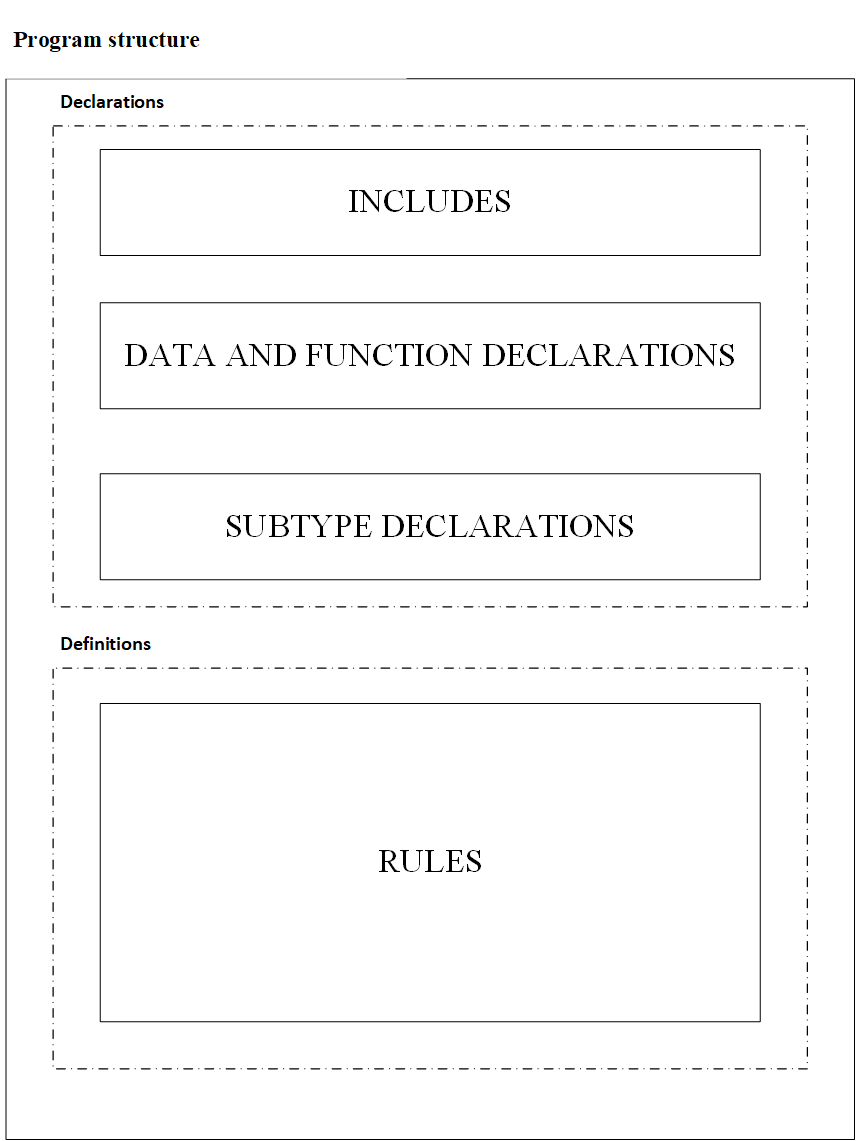
\includegraphics[width = 0.6\textwidth]{Figures/chapter_metacasanova/program_structure}
	\caption{Structure of a program in Metacasanova}
	\label{fig:ch_metacasanova_program_structure}
\end{figure}

\begin{comment}
\subsection{Syntax in BNF}
The following is the syntax of Metacasanova in Backus-Naur form. Note that, for brevity, we omit the definitions of typical syntactical elements of programming languages, such as literals or identifiers:

\begin{lstlisting}[basicstyle = \ttfamily\tiny]
<program> ::= 
{<include>} {<import>} {<data>} <function> {<function>} {<alias>} <rule> {<rule>}
<premise> ::= 
<clause> | <functionCall> | <binding>
<binding> ::= 
id ":=" <constructor>
<rule> ::= 
{premise} "-" {"-"} <functionCall>
<clause> ::= //typical boolean expression
<functionCall> ::= 
<id> {<argument>} <arrow> <argument> | 
{<argument>} <id> {<argument>} <arrow> <argument> | 
<id> {<argument>} <arrow> <argument>
<arrow> ::= "=>" | "==>"
<constructor> ::= 
<id> {<argument>} | 
{<argument>} <id> {<argument>} | 
{<argument>} <id>
<external> ::= "<<" <csharpexpr> ">>"
<csharpexpr> ::= //all available C# expressions
<argument> ::= 
["("] 
(<id> | 
<external> | 
<literal> | 
<constructor>) 
[")"]
<literal> ::= //typical literals such as integer, float, string, ...
<import> ::= import id {"." id}
<include> ::= include id {.id}
<alias> ::= <typeDef> is <typeDef>
<typeDef> ::= id | "<<" id ">>"
<typeArguments> :: = 
'"' <id> '"' {"->" <typeDef>} ":" <typeDef> |
<typeDef> {"->" <typeDef>} "->" '"' <id> '"' {"->" <typeDef>} ":" <typeDef> |
<typeDef> {"->" typeDef} "->" '"' <id> '"' ":" <typeDef> 
<function> ::= Func <typeArguments> "=>" <typeDef> [Priority <literal>]
<data> ::= Data <typeArguments> [Priority <literal>]
\end{lstlisting}
\end{comment}

\subsection{Formalization}
In what follows we assume that the pattern matching of the function arguments in a rule succeeds, otherwise a rule will fail to return a result.
The informal semantics of the rule evaluation in Metacasanova is the following:
\begin{enumerate}
	\item[R1] A rule with no clauses or function calls always returns a result.
	\item[R2] A rule returns a result if all the clauses evaluate to \texttt{true} and all the function calls in the premise return a result.
	\item[R3] A rule fails if at least one clause evaluates to \texttt{false} or one of the function calls fails (returning no results).
\end{enumerate}
We will express the semantics, as usual, in the form of logical rules, where the conclusion is obtained when all the premises are true.
In what follows we consider a set of rules defined in the Metacasanova language $R$. Each rule has a set of function calls $F$ and a set of clauses (boolean expressions) $C$. We use the notation $f^{r}$ to express the application of the function $f$ through the rule $r$. We will define the semantics by using the notation $\langle expr \rangle$ to mark the evaluation of an expression, for example $\langle f^{r} \rangle$ means evaluating the application of $f$ through $r$. The following is the formal semantics of the rule evaluation in Metacasanova, based on the informal behaviour defined above:


\begin{mathpar}
	\mprset{flushleft}
	\inferrule*[left=R1:]
	{C = \emptyset \\\\ F = \emptyset}
	{\langle f^{r} \rangle \Rightarrow \lbrace x \rbrace} \\
	
	\mprset{flushleft}
	\inferrule*[left=R2:]
	{\forall c_{i} \in C \;, \langle c_{i} \rangle \Rightarrow true \\\\
		\forall f_{j} \in F \; , \exists r_{k} \in R \; | \; \langle f_{j}^{r_{k}} \rangle \Rightarrow \lbrace x_{r^{k}} \rbrace}
	{\langle f^{r} \rangle \Rightarrow \lbrace x_{r} \rbrace} \\
	
	\mprset{flushleft}
	\inferrule*[left=R3(a):]
	{\exists c_{i} \in C \; | \; \langle c_{i} \rangle \Rightarrow false}
	{\langle f^{r} \rangle \Rightarrow \emptyset} \\
	
	\mprset{flushleft}
	\inferrule*[left=R3(b)]
	{\forall r_{k} \in R \; , \exists f_{j} \in F \; | \; \langle f_{j}^{r_{k}} \rangle \Rightarrow \emptyset}
	{\langle f^{r} \rangle \Rightarrow \emptyset}
\end{mathpar}

R1 says that, when both $C$ and $F$ are empty (we do not have any clauses or function calls), the rule in Metacasanova returns a result. R2 says that, if all the clauses in $C$ evaluates to true and, for all the function calls in $F$ we can find a rule that returns a result (all the function applications return a result for at least one rule of the program), then the current rule returns a result. R3(a) and R3(b) specify when a rule fails to return a result: this happens when at least one of the clauses in $C$ evaluates to false, or when one of the function applications does not return a result for any of the rules defined in the program.

\section{Architectural overview}
\label{sec:ch_metacasanova_architecture}
In this section we provide a general overview of the architecture of Metacasanova compiler.

The compiler has a modular structure: in the front-end we find the the lexer/parser and a parser post-processing module. The latter is required because not all information necessary to build all the elements of the AST is immediately available during the parsing phase. For instance, some data structures store the file name that is being compiled and the name of the current module, but this information is available only after the parsing itself. 

The generated AST is passed to the type checker to check the type correctness. Note that the type checker of the metacompiler checks the meta-types, i.e. the types defined in the meta-program, and not the types of the terms of the language that is being implemented in Metacasanova. This module checks the correctness of the declarations and the terms used in rules. The type checker outputs a data structure containing information about the types of the declarations and terms used in rules (in short a \textit{typed program definition}).

The output of the AST is passed to the code generator that uses information about the types to correctly generate the target code. This is needed because Metacasanova generates C\# code, which is a typed high-level language that requires information about the types to define variables, methods, and classes representing the elements of the meta-program.

Note that also, with this implementation choice, it is possible to support different high-level programming languages, both typed and untyped: the only component that changes will be the generation of the behaviour of the rules in the abstractions provided by the different target languages. A possible improvement of this architecture is generating a common intermediate language that is later translated into the target code, but this falls outside the scope of this work.


\section{Parsing}
\label{sec:ch_metacasanova_parsing}
In this section we explain in detail the grammar of Metacasanova and we present the architecture of its parser. The parser has been built in FsYacc (see Section \ref{sec:ch_background_parser_generators}) and completed by a post-processing module that executes some required transformation on the generated AST that are not convenient to perform during the parsing phase. As explained informally in Section \ref{sec:ch_metacasanova_metacasanova_overview}, a Metacasanova program is made of four main sections: (\textit{i}) a part containing inclusion directives, (\textit{ii}) a part containing the declarations of the meta-data stracutures and evaluation functions used in the program, (\textit{iv}) a part containing type equivalences, and (\textit{iii}) a part containing evaluation rules that define the behaviour of the meta-program. The definition of the first part is trivial and we do not examine it in detail. We will instead describe in detail the other parts.
	
\subsection{Declarations}
\label{sec:ch_metacasanova_parser_declarations}
Declarations contain \textit{function} or \textit{data} declarations. A meta-data structure is a meta-language representation of an abstraction of the language implemented in the metacompiler and contains both syntactical and structural information. For example, an arithmetic operator in a programming language can be represented as a meta-data structure containing both its symbol and the values of its arugments. Meta-data structures can be recursive, i.e. it is possible to have arguments that are instances of the same meta-data structure. This is done in order to allow recursive data structures such as lists. A meta-data structure declaration begins with the keyword \texttt{Data} and is followed by a series of arguments, which are separated by arrows, that can be both type names and strings representing the name of the meta-data. It is possible to declare an infix or suffix operator by placing its name after the first position of the arguments. For instance, the following code defines a sum operator for arithmetic expressions with an infix notation.

\begin{lstlisting}
Data Expr -> "+" -> Expr : Expr
\end{lstlisting}

Type names are identifier that begins with an alphabetic character followed by one or more alphanumeric characters or underscores. The regular expression defining this syntax is expressed as

\begin{lstlisting}
ID ::= ['a'-'z' 'A'-'Z'] ['a'-'z' 'A'-'Z' '_' '0'-'9']+
\end{lstlisting}

Type names can also contain external code enclosed by double angular brackets to make use of external types such as .NET primitive types (\texttt{int}, \texttt{float}, etc.). The operator names are strings that may contain any symbol usually allowed in strings in usual programming languages.

The arguments are followed by a type name defining the type of the meta-data structure. Optionally it is possible to specify a priority and the associativity, otherwise the default priority will be -1 and the operator will be left-associative.

Function declarations have the same structure except they begin with the keyword \texttt{Func} instead.

Both data and function declarations may define generic arguments. In order to specify generic arguments, they must be enclosed between square brackets after the declaration keyword. For instance the following code defines a data structure representing a tuple

\begin{lstlisting}
Data[a,b] a -> "," -> b : Tuple[a,b]
\end{lstlisting}

Finally, each declaration must end with a line break. Line breaks are used in Metacasanova to separate different language elements, as in this case.

The grammar production used to describe the syntax of declarations is the following:

\begin{lstlisting}
declaration:
| FUNC genericSeq typeOrNameDeclarations COLON typeDeclaration priority associativity newLineSeq {
Func(processParsedArgs $3 $5 (fst $1) (snd $1) $2 $6 $7) }
| DATA genericSeq typeOrNameDeclarations COLON typeDeclaration priority associativity newLineSeq {
Data(processParsedArgs $3 $5 (fst $1) (snd $1) $2 $6 $7) }
\end{lstlisting}

Since type names and data or function names can appear in any order, the parser generates a support polymorphic data structure in F\#.

\begin{lstlisting}
type TypeDeclOrName =
| Type of TypeDecl
| Name of string
\end{lstlisting}

This data structure is later transformed by the parser post-processor in a \textit{symbol declaration}. A symbol declaration contains all the information about a declaration, including the data or function name, the types of the arguments, the priority, and the generic types. This information is later exploited by the type checker to verify the consistency of the declarations and type check the rest of the program.

\subsubsection{Type equivalence declarations}
Type equivalence has been presented as a separate part of the program but it has a tight relationship with the declarations. A type equivalence has the form

\begin{lstlisting}
T1 is T2
\end{lstlisting}

where T1 and T2 are two meta-type names. They are used to specify that meta-type T1 is equivalent to meta-type T2 and can replace any argument of type T2 while constructing meta-data structures or calling functions. The grammar rule that defines a type equivalence declaration is

\begin{lstlisting}
ID IS ID newLineSeq
\end{lstlisting}

\noindent
where \texttt{ID} is the same regular expression used for type names. Again successive equivalence declarations should be separated by one or more line breaks. The grammar production generates a list of pairs in the AST containing the types involved in the equivalence. This data structure will be processed at a later stage by the type checker to generate an equivalence table.

\subsection{Rules}
\label{sec:ch_metacasanova_parser_rules}
Rules in Metacasanova are the language elements used to define the behaviour of the meta-program. A rule consists of a set of premises followed by a conclusion. Premises and conclusion are separated by a fraction line. Premises and conclusion are made of a left part consisting of a sequence of arguments, and a right part that can contain either a variable or a sequence of arguments. We call the left part of this syntactical structure \textit{function call}, while the right part is the \textit{result}. Premises differ from the conclusion as, besides function calls, they can also contain \textit{bindings} and \textit{clause}. Bindings are simply ways to rename values in the premises in the fashion of bindings in functional languages, while clauses are boolean predicates. Moreover, premises can also contain .NET code to directly emit, which can contain any C\# code. The syntax of emitted code is the same as that of a normal premise, except the \textit{function call} is replaced by the code to emit enclosed in double angular brackets. The following is the grammar production defining a premise\footnote{ \texttt{BIND} is the symbol \texttt{:=}}:

\begin{lstlisting}
premise:
| emit premises { $1 :: $2 }
| functionCall premises { $1 :: $2 }
| ID BIND arg newLineSeq premises { (Bind({ Namespace = ""; Name = fst $1 },Position.Create(snd $1,""),$3)) :: $5 }
| arg comparisonOp arg newLineSeq premises { (Conditional($1,$2,$3)) :: $5 }
| { [] }

functionCall:
| argSeq ARROW argSeq newLineSeq { FunctionCall($1,$3) }
\end{lstlisting}

Note that premises are optional (axioms do not have any premise in a logical rule), so an empty list is returned when none is given. Note that the namespace required for variables, such as in the binding, is left empty because at this point the namespace of the program is not available yet. The namespace will be later filled in by the parser post-processor. Also note that, in this stage, we do not check if each function call actually contains a function name, and we simply parse a premise (and a conclusion) as a sequence of arguments, that could be function or data names, variables, literals, or nested expressions. Nested expressions are expressions enclosed in brackets and are themselves other sequences of arguments. The actual control that premises and conclusions contain a function name is performed by the type checker, because to correctly identify the function name a complete symbol table, unavailable in this moment, is required. A conclusion has the same syntax of a function call:

\begin{lstlisting}
conclusion:
| argSeq ARROW argSeq newLineSeq { ValueOutput($1,$3) }
\end{lstlisting}

The parser generates a data structure for a rule containing a representation of the premises and the conclusion:

\begin{itemize}[noitemsep]
\item \textit{function call}: A function call is simply a pair of list of arguments, where the left element is the call itself, while the right element is the result.

\item \textit{emit}: Emitted code contains the code in string format and the variable it is assigned to (used to save the result of expressions or function calls).

\item \textit{bind}: Bindings contain the variable name used for the binding and its argument, which can be a literal, the constructor of a meta-data structure, or another variable.

\item \textit{conditional}: Conditionals are boolean expressions that may contain comparison operators. Their representation stores their left and right argument and the comparison operator.
\end{itemize}

\subsection{Parser post-processor}
\label{sec:ch_metacasanova_parser_post-processor}

\section{Type checking}

\section{Code generation}

\subsection{Data structures code generation}
The type of each data structure is generated as an interface in C\#. Each data structure defined in Metacasanova is mapped to a \texttt{class} in C\# that implements such interface. The class contains as many fields as the number of arguments the data structure contains. Each field is given an automatic name \texttt{argC} where \texttt{C} is the index of the argument in the data structure definition. The data structure symbols used in the definition might be pre-processed and replaced in order to avoid illegal characters in the C\# class definition. The class contains an additional field that stores the original name of the data structure before the replacement is performed, used for its ``pretty print''. For example the data structure

\begin{lstlisting}
Data "$i" -> int : Value
\end{lstlisting}

\noindent
will be generated as

\begin{lstlisting}
public interface Value {  }

public class __opDollari : Value
{
public string __name = "$i";
public int __arg0;

public override string ToString()
{
return "(" + __name + " " + __arg0 + ")";
}
}
\end{lstlisting}

\subsection{Code generation for rules}
Each rule contains a set of premises that in general call different functions to produce a result, and a conclusion that contains the function evaluated by the current rule and the result it produces. The code generation for the rules follows the steps below:

\begin{enumerate}
	\item Generate a data structure for each function defined in the meta-program.
	\item For each function $f$ extract all the rules whose conclusion contains $f$.
	\item Create a \texttt{switch} statement with a case for each rule that is able to execute the function (the function is in its conclusion).
	\item In the case block of each rule, define the local variables defined in the rule.
	\item Apply pattern matching to the arguments of the function contained in the conclusion of the rule. If it fails, jump immediately to the next case (rule).
	\item Store the values passed to the function call into the appropriate local variables.
	\item Run each premise by instantiating the class for the function used by it and copying the values into the input arguments.
	\item Check if the premise outputs a result and, in the case of an explicit data structure argument, check the pattern matching. If the premise result is empty or the pattern matching fails for all the possible executions of the premise then jump to the next case.
	\item Generate the result for the current rule execution. 
\end{enumerate}

\noindent
In what follows, we use as an example the code generation for the following rule (which computes the sum of two integer expressions in a programming language):

\begin{lstlisting}
eval a -> $i c
eval b -> $i d
<< c + d >> -> e
----------------
eval (a + b) -> $i e
\end{lstlisting}

From now on we will refer to an argument as \textit{explicit data argument} when its structure appears explicitly in the conclusion or in one of the premises, as in the case of \texttt{a + b} in the example above.

\subsubsection{Data structure for the function}
\label{subsubsec:function_generation}

As first step the meta-compiler generates a class for each function defined in the meta-program. This class contains one field for each argument the function accepts. It also contains a field to store the possible result of its evaluation. This field is a \texttt{struct} generated by the meta-compiler defined as follows:

\begin{lstlisting}
public struct __MetaCnvResult<T> { public T Value; public bool HasValue; }
\end{lstlisting}

The result contains a boolean to mark if the rule actually returned a result or failed, and a value which contains the result in case of success.

For example, the function

\begin{lstlisting}
Func eval -> Expr : Value
\end{lstlisting}

\noindent
will be generated as

\begin{lstlisting}
public class eval
{
public Expr __arg0;
public __MetaCnvResult<Value> __res;
...
}
\end{lstlisting}

\subsubsection{Rule execution}

The class defines a method \texttt{Run} that performs the actual code execution. The meta-compiler retrieves all the rules whose conclusion contains a call to the current function, which define all the possible ways the function can be evaluated with. It then creates a \texttt{switch} structure where each \texttt{case} represents each rule that might execute that function. The result of the rule is also initialized here (the \texttt{struct} will contain a default value and the boolean flag will be set to \texttt{false}). Each \texttt{case} defines a set of local variables, that are the variables used within the scope of that rule.

\subsubsection{Local variables definitions and pattern matching of the conclusion}

At the beginning of each \texttt{case}, the meta-compiler defines the local variables initialized with their respective default values. It also generates then the code necessary for the pattern-matching of the conclusion arguments. Since variables always pass the pattern-matching, the code is generated only for arguments explicitly defining a data structure (see the examples about arithmetic operators in Section \ref{sec:semantics}) and literals. If the pattern matching fails then the execution jumps to the next \texttt{case} (rule). For instance, the code for the following conclusion

\begin{lstlisting}
...
-------------
eval (a + b) -> $i e
\end{lstlisting}

\noindent
is generated as follows

\begin{lstlisting}
case 0:
{
Expr a = default(Expr);
Expr b = default(Expr);
int c = default(int);
int d = default(int);
int e = default(int);
if (!(__arg0 is __opPlus)) goto case 1;
...
}
\end{lstlisting}

\noindent
Note that an explicit data argument, such in the example above, might contain other nested explicit data arguments, so the pattern-matching is recursively performed on the data structure arguments themselves.

\subsubsection{Copying the input values into the local variables}
When each function is called by a premise, the local values are stored into the class fields of the function defined in Section \ref{subsubsec:function_generation}. These values must be copied to the local variables defined in the \texttt{case} block representing the rule. Particular care must be taken when one argument is an explicit data. In that case, we must copy, one by one, the content of the data into the local variables bound in the pattern matching. For example, in the rule above, we must separately copy the content of the first and second parameter of the explicit data argument into the local variables \texttt{a} and \texttt{b}. The generated code for this step, applied to the example above, will be:

\begin{lstlisting}
__opPlus __tmp0 = (__opPlus)__arg0;
a = __tmp0.__arg0;
b = __tmp0.__arg1;
\end{lstlisting}

Note that the type conversion from the polymorphic type \texttt{Expr} into \texttt{opPlus} is now safe because we have already checked during the pattern matching that we actually have \texttt{opPlus}.

\subsubsection{Generation of premises}
Before evaluating each premise, we must instantiate the class for the function that they are invoking. The input arguments of the function call must be copied into the fields of the instantiated object. If one of the arguments is an explicit data argument, then it must be instantiated and its arguments should be initialized, and then the whole data argument must be assigned to the respective function field. After this step, it is possible to invoke the \texttt{Run} method of the function to start its execution. The first premise of the example above then becomes (the generation of the second is analogous):

\begin{lstlisting}
eval a -> $i c
\end{lstlisting}

\begin{lstlisting}
eval __tmp1 = new eval();
__tmp1.__arg0 = a;
__tmp1.Run();
\end{lstlisting}

\subsubsection{Checking the premise result}
After the execution of the function called by a premise, we must check if a rule was able to correctly evaluate it. In order to do so, we must check that the result field of the function object contains a value, and if not the rule fails and we jump to the next case (rule), which is performed in the following way:

\begin{lstlisting}
if (!(__tmp1.__res.HasValue)) goto case 1;
\end{lstlisting}

If the premise was successfully evaluated by one rule, then we must check the structure of the result, which leads to the following three situations:
\begin{enumerate}
	\item The result is bound to a variable.
	\item The result is constrained to be a literal.
	\item The result is an explicit data argument.
\end{enumerate}

In the first case, as already explained above, the pattern matching always succeeds, so no check is needed. In the second case, it is enough to check the value of the literal. In the last case, all the arguments of the data argument must be checked to see if they match the expected result. In general this process is recursive, as the arguments could be themselves other explicit data arguments. If the result passes the check, then the result is copied into the local variables, in a fashion similar to the one performed for the function premise. For instance, for the premise

\begin{lstlisting}
eval a -> $i c
\end{lstlisting}

\noindent
the meta-compiler generates the following code to check the result
\begin{lstlisting}
if (!(__tmp1.__res.Value is __opDollari)) goto case 1;
__MetaCnvResult<Value> __tmp2 = __tmp1.__res;
__opDollari __tmp3 = (__opDollari)__tmp2.Value;
c = __tmp3.__arg0;
\end{lstlisting}

\subsubsection{Generation of the result}
When all premises correctly output the expected result, the rule can output the final result. In order to do that, the generated code must copy the right part of the conclusion (the result) into the \texttt{res} variable of the function class. If the right part of the conclusion is, again, an explicit data argument, then the data object must first be instantiated and then copied into the result. For example the result of the rule above is generated as follows:

\begin{lstlisting}
res = c + d;
__opDollari __tmp7 = new __opDollari();
__tmp7.__arg0 = res;
__res.HasValue = true;
__res.Value = __tmp7;
break;
\end{lstlisting}

\noindent
After this step, the rule evaluation successfully returns a result.

This implementation choice is due to the fact that we plan to support partial function applications, thus, when a function is partially applied, there is the need to store the values of the arguments that were partially given. This could still be implemented with static methods and lambdas in C\#, but not all programming languages natively support lambda abstractions, so we chose to have a set-up that allows us to change the target language without dramatically altering the logic of code generation.


